%------------------------------------------------------------------------Begin preamble------------------------------------------------------------------------
\documentclass[12pt]{article}
% Uncomment these two lines if you want to use Times New Roman (needs XeLaTeX)
% \usepackage{fontspec}
% \setmainfont{Times New Roman}

\usepackage{amsmath} % For math
\usepackage{amssymb} % For more math
\usepackage{fancyhdr} % For fancy headers and footers
\usepackage{fancyvrb} % For writing blocks of code verbatim (like LaTeX code)
\usepackage{geometry} % For manipulating margins and meta doc stuff
\usepackage{graphicx} % Required for inserting images
\usepackage{hyperref} % For linking stuff
\usepackage{cleveref} % Better cross refencing % Must be loaded after hyperref
\usepackage{lastpage} % For doing "Page n of |n|"
\usepackage{minted} % For color coding code sections
\usepackage{pgfplots} % For adding plots and graphs
\usepackage[indent=00pt]{parskip} % Get rid of beginning indents on paragraphs and set spacing between paragraphs
\usepackage{siunitx} % For adding siunits inside math zones
\usepackage[most]{tcolorbox} % For inserting color boxes
\usepackage{tikz}
\usepackage{titling} % For vertically centering title, author, and date
\usepackage{tocloft} % For cooler toc
\usepackage{xcolor} % For coloring text
\usepackage{witharrows} % For cool arrows for pointing at stuff

%%%%%%%%% Begin tocloft setup %%%%%%%%%%%%%%
\renewcommand\cftsecfont{\normalfont}
\renewcommand\cftsecpagefont{\normalfont}
\renewcommand{\cftsecleader}{\cftdotfill{\cftsecdotsep}}
\renewcommand\cftsecdotsep{\cftdot}
\renewcommand\cftsubsecdotsep{\cftdot}
%%%%%%%%% End tocloft %%%%%%%%%%%%%%

%%%%%%%%%% Begin hyperref setup %%%%%%%%%%%%%%%%%%%
\hypersetup{
    colorlinks=true,
    linkcolor=blue,
    urlcolor=blue,
}
%%%%%%%%%% End hyperref setup %%%%%%%%%%%%%%%%%%%

%%%%%%% Begin pgfplotsset setup %%%%%%%
\pgfplotsset{compat=1.18} % Compiler be bugging
%%%%%%% End pgfplotsset setup %%%%%%%

%%%%%%% Begin fancyhdr setup %%%%%%%
\pagestyle{fancy}
\renewcommand{\footrulewidth}{0.4pt} % default is 0pt
\lhead{Linear Algebra} % Top left header
\chead{} % Top center header
\rhead{} % Top right header

\lfoot{Brandon J. T. Noguera} % Bottom left footer
\cfoot{} % Bottom center footer
\rfoot{Page \thepage\ of \pageref*{LastPage}} % Bottom right footer
% doing \pageref*{some_url} turns off the hyperlink capability for some_url
%%%%%%% End fancyhdr setup %%%%%%%

%%%%%%% Begin titlingpage setup %%%%%%%
\renewcommand\maketitlehooka{\null\mbox{}\vfill}
\renewcommand\maketitlehookd{\vfill\null}
%%%%%% End titlingpage setup %%%%%%%
%------------------------------------------------------------------------End preamble------------------------------------------------------------------------

\title{\textbf{Linear Algebra}}
\author{Brandon Jose Tenorio Noguera}
\begin{document}

\begin{titlingpage}
\maketitle
\end{titlingpage}

\tableofcontents
\newpage

\section{Sources}\label{srcs}
\begin{tcolorbox}[title=Sources]
These notes were taking from \href{https://ocw.mit.edu/courses/18-06sc-linear-algebra-fall-2011/pages/syllabus/}{MIT Linear Algebra taught by Professor Gilbert Strang} and \href{https://ocw.mit.edu/courses/res-18-010-a-2020-vision-of-linear-algebra-spring-2020/}{MIT A Vision of Linear Algbera by Professor Gilbert Strang}
\end{tcolorbox}

\section{Course goals}\label{}

After completing this course, you will understand:
\begin{itemize}
  \item Systems of linear equations
  \item Row reduction and echelon forms
  \item Matrix operations, including inverses
  \item Block matrices
  \item Linear dependece and independence
  \item Subspaces and bases and dimensions
  \item Orthogonal bases and orthogonal projections
  \item Gram-Schmidt process
  \item Linear models and least-squares problems
  \item Determinants and their properties
  \item Cramer's Rule
  \item Eqigenvalues and eigenvectors
  \item Diagonalization of a matrix
  \item Symmetric matrices
  \item Positive definite matrices
  \item Similar matrices
  \item Linear transformations
  \item Singular value decomposition
  
\end{itemize}

\section{Unit I: Ax = b and the Four Subspaces}\label{u1}

\subsection{The Geometry of Linear Equations}\label{u1.1}


Imagine you're given $n $ linear equations with $n $ linear unknowns. In linear algebra you can look at (or think of) this system in one of three ways:
\begin{itemize}
    \item Row picutre
    \item Column picture
    \item Matrix form
\end{itemize}

Example: imagine we're given this system of linear equations
\begin{align*}
    2x - y &= 0\\
    -x + 2y &= 3\\
\end{align*}

If we think of this in \textbf{matrix form} we get...
\begin{align*}
  \begin{bmatrix}
    2 & -1\\
    -1 & 2
  \end{bmatrix}
  \begin{bmatrix}
  x\\
  y
  \end{bmatrix}
  &= 
  \begin{bmatrix}
  0\\
  3
  \end{bmatrix}\\
\end{align*}
Which we can generalize like...
\begin{align*}
  Ax &= b\\
\end{align*}
Where
\begin{align*}
  A &= \text{ matrix of coefficients}\\
  x &= \text{ matrix of unknowns}\\
  b &= \text{ matrix of constants }\\
\end{align*}
If we think of this in \textbf{row picture form} we get a graph with $x $ and $y $ coordinates that satisfy each equation like...

\begin{align*}
  \begin{tikzpicture}
    \begin{axis}[
      xmin=-5,
      xmax=5,
      ymin=-5,
      ymax=5,
      axis lines=middle,
      xlabel=$ x $,
      ylabel=$ y $,
      title={Row picture},
      xmajorgrids=true,
      ymajorgrids=true,
      grid style=dashed,
      domain=-5:5,
      ]
      \addplot [blue] {2*x***REMOVED*** 
      \addplot [red] {(x+3)/2***REMOVED***
    \end{axis}
  \end{tikzpicture}\\
\end{align*}
Where the \textcolor{blue}{\textbf{blue line}} represents $ 2x-y=0 $ and the \textcolor{red}{\textbf{red line}} represents $ -x+2y=3 $


If we think of this in \textbf{column picture form} we get the following equation
\begin{align*}
  x \cdot \begin{bmatrix}
    2\\
    -1
  \end{bmatrix}
  +
  y \cdot \begin{bmatrix}
    -1\\
    2
  \end{bmatrix}
  =
  \begin{bmatrix}
    0\\
    3
  \end{bmatrix}\\
\end{align*}
Which we refer to as the \textbf{linear combination} of the columns.
This can be represented as a vector graph like so

\begin{align*}
  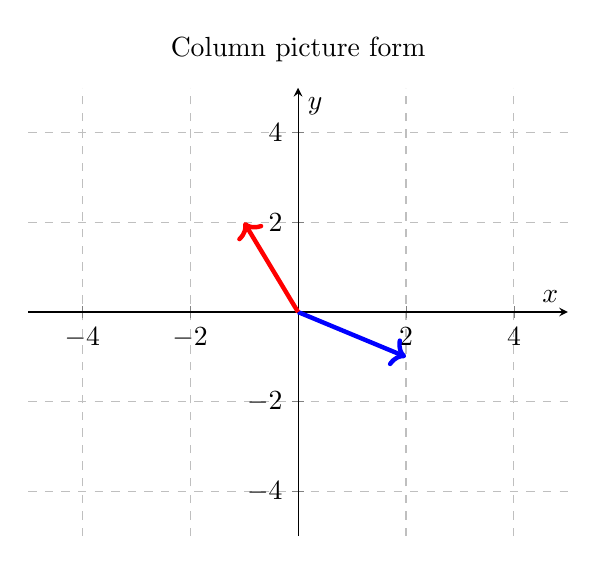
\begin{tikzpicture}
    \begin{axis}[
      xmin=-5,
      xmax=5,
      ymin=-5,
      ymax=5,
      axis lines=middle,
      xlabel=$ x $,
      ylabel=$ y $,
      title={Column picture form},
      xmajorgrids=true,
      ymajorgrids=true,
      grid style=dashed,
      domain=5:5,
      ]
      \draw[ultra thick, blue, ->] (0,0) -- (2,-1);
      \draw[ultra thick, red, ->] (0,0) -- (-1,2);
    \end{axis}
  \end{tikzpicture}
\end{align*}

Where the \textcolor{blue}{\textbf{blue}} vector represents the column \begin{equation*}
  \begin{bmatrix}
  2\\
  -1
  \end{bmatrix}
\end{equation*}
and the \textcolor{red}{\textbf{red}} vector represents the column \begin{equation*}
  \begin{bmatrix}
  -1\\
  2
  \end{bmatrix}
\end{equation*}

Now we need to take a combination. Let $x=1 $ and $y=2 $

\begin{align*}
    1 \begin{bmatrix}
    2\\
    -1
    \end{bmatrix}
    +
    2 \begin{bmatrix}
    -1\\
    2
    \end{bmatrix}
    =
    \begin{bmatrix}
    0\\
    3
    \end{bmatrix}
\end{align*}

\begin{align*}
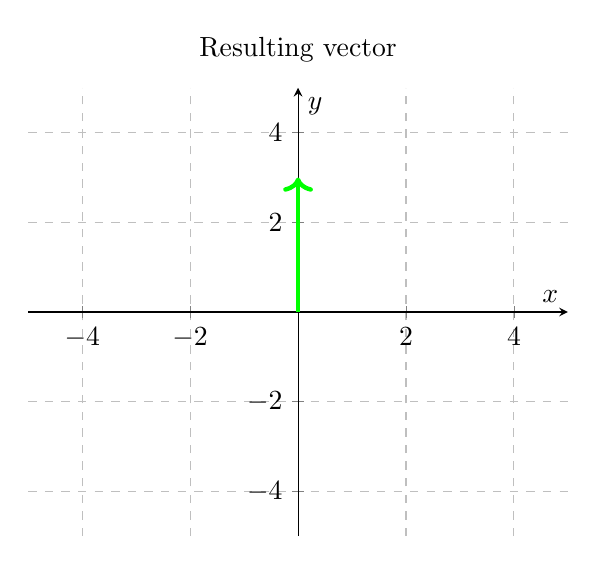
\begin{tikzpicture}
  \begin{axis}[
    xmin=-5,
    xmax=5,
    ymin=-5,
    ymax=5,
    axis lines=middle,
    xlabel=$ x $,
    ylabel=$ y $,
    title={Resulting vector},
    xmajorgrids=true,
    ymajorgrids=true,
    grid style=dashed,
    domain=5:5,
    ]
    \draw[ultra thick, green, ->] (0,0) -- (0,3);
  \end{axis}
\end{tikzpicture}
\end{align*}

What are all the combination of $ x $ and $ y $ that satisfy this equation?

Another example. Assume we're given this system of linear equations:

\begin{align*}
    2x-y+0z &= 0\\
    -x + y - z &= -1\\
    0x - 3y + 4z &= 4
\end{align*}

In matrix for we get
\begin{align*}
    A &= \begin{bmatrix}
      2 & -1 & 0\\
      -1 & 2 & -1\\
      0 & -3 & 4 
    \end{bmatrix}
    =
    \begin{bmatrix}
    0\\
    -1\\
    4
    \end{bmatrix}
\end{align*}

In row picture form we get

% TODO add a 3d graph
% \begin{align*}
% \begin{tikzpicture}
%   \begin{axis}[
%     xmin=-10,
%     xmax=10,
%     ymin=-10,
%     ymax=10,
%     axis lines=middle,
%     xlabel=$ x $,
%     ylabel=$ y $,
%     title={graph title},
%     xmajorgrids=true,
%     ymajorgrids=true,
%     grid style=dashed,
%     domain=10:10,
%     ]
%     
%   \end{axis}
% \end{tikzpicture}
% \end{align*}

Steps to solve in row picture form:
\begin{itemize}
    \item Find all the points that would satisfy this equation
    \item In our example, some solutions would be: 
    \begin{itemize}
        \item $ (x=1, y=0, z=0) $
        \item $ (z=1, x=0, y=0) $ 
        \item $ (x=0, z=0, y=-\frac{1}{2}) $
    \end{itemize}
\end{itemize}

Each row in a 3 by 3 gives us a plane in 3 dimensions. Those planes meet in one points, and that's the solution

\textbf{Column picture form}

\begin{align*}
    x \begin{bmatrix}
    2\\
    -1\\
    0
    \end{bmatrix}
    +
    y \begin{bmatrix}
    -1\\
    2\\
    -3
    \end{bmatrix}
    + z \begin{bmatrix}
    0\\
    -1\\
    4
    \end{bmatrix}
    = \begin{bmatrix}
    0\\
    -1\\
    4
    \end{bmatrix}
\end{align*}

We want to know what combination of the \textbf{left hand} vectors produces the \textbf{right hand vector}

% TODO draw 3d vector graph for this

It is obvious that the $ z $ vector is one combination that solves this system. So if we let $ x=0, y=0, z=1 $ we have found our answer!

Now imagine the system looks like this

\begin{align*}
    x \begin{bmatrix}
    2\\
    -1\\
    0
    \end{bmatrix}
    +
    y \begin{bmatrix}
    -1\\
    2\\
    -3
    \end{bmatrix}
    + z \begin{bmatrix}
    0\\
    -1\\
    4
    \end{bmatrix}
    = \begin{bmatrix}
    1\\
    1\\
    -3
    \end{bmatrix}
\end{align*}

Now we've built the right hand vector by letting $ x=1, y=1, z=0 $, and that would be one of our solutions!

Now, is it possible to \textbf{solve Ax=b for every b?}.

Changing the wording, we can ask: \emph{do the \textbf{lniear combinations of the columns} fill 3 dimensional space?}

For the matrix $ A $ above, the answer is yes! 

Let's think, when would the right hand vector not be produceable? If the 3 columns lie on the \textbf{same plane}, we would not be able to get the right vector. In other words, if one column was exactly the same as another column, we may not be able to get $ b $

\begin{align*}
    Ax &= b
\end{align*}

How to multiply a matrix by a vector?

\begin{align*}
    \begin{bmatrix}
      2 & 5\\
      1 & 3
    \end{bmatrix}
    \begin{bmatrix}
    1\\
    2
    \end{bmatrix}
    &= 
    1 \begin{bmatrix}
    2\\
    1
    \end{bmatrix}
    +
    2 \begin{bmatrix}
    5\\
    3
    \end{bmatrix}
    = \begin{bmatrix}
    1(2) + 2(5) = 12\\
    1(1) + 2(3) = 7
    \end{bmatrix}
\end{align*}

$Ax$ is a combination of the columns of $ A $

\subsection{An Overview of Key Ideas}\label{}











































\end{document}
